\documentclass[12pt]{article}

\usepackage{geometry}
\usepackage{graphicx}
\usepackage{amsmath}
\usepackage{amssymb}
\usepackage{lscape}
\usepackage[table,svgnames, dvipsnames]{xcolor}
\usepackage{color}
\usepackage{pgfgantt}
\usepackage{array}
\usepackage{appendix}
\usepackage{setspace}
\usepackage{listings}
\usepackage[toc,page]{appendix}
\usepackage{tikz, pgfplots}
\usetikzlibrary{positioning}

\usepackage[colorlinks]{hyperref}
\usepackage[symbols,nogroupskip,sort=use]{glossaries-extra}

\makenoidxglossaries
\glsxtrnewsymbol[description={Caputo Derivative}]{caputo_derivative}{\ensuremath{_{c}D^{\alpha}}}
\glsxtrnewsymbol[description={Riemann-Liouville Derivative}]{riemann_liouville_derivative}{\ensuremath{_{rl}D^{\alpha}}}
\glsxtrnewsymbol[description={Gr\"{u}nwald-Letnikov}]{grunwald_letnikov_derivative}{\ensuremath{_{gl}D^{\alpha}}}
\glsxtrnewsymbol[description={General Dependent Variable}]{general_dependent_variable}{\ensuremath{x}}
\glsxtrnewsymbol[description={Time Step}]{time_step}{\ensuremath{h}}
\glsxtrnewsymbol[description={Time Step Index}]{time_step_index}{\ensuremath{k}}
\glsxtrnewsymbol[description={General Function}]{general_function}{\ensuremath{f(x)}}
\glsxtrnewsymbol[description={General First Order Derivative Of Function $f(x)$}]{first_order}{\ensuremath{f^{\prime}(x)}}
\glsxtrnewsymbol[description={General Second Order Derivative Of Function $f(x)$}]{second_order}{\ensuremath{f^{\prime\prime}(x)}}
\glsxtrnewsymbol[description={General $n$th Order Derivative Of Function $f(x)$}]{general_order_derivative}{\ensuremath{f^{(n)}(x)}}

\graphicspath{ {./images/} }

\newcommand\tab[1][1cm]{\hspace*{#1}}

\newenvironment{conditions}
  {\par\vspace{\abovedisplayskip}\noindent\begin{tabular}{>{$}l<{$} @{${}={}$} l}}
  {\end{tabular}\par\vspace{\belowdisplayskip}}

\geometry{margin=1.2in}

\onehalfspacing

\begin{document}

\begin{titlepage}
	\begin{center}
        \vspace*{1cm}
            
        \Huge
        \textbf{Modelling and administration of chemo-therapeutics for the treatment of ovarian cancer}
            
        \vspace{0.5cm}
        \Huge
        MEng (Hons) Final Year Project Report
            
        \vspace{1.5cm}
        
        \Large    
        \textbf{Student Name: Daniel Bradley}\\
        \textbf{Supervisor: Dr Pantelis Sopasakis}
            
        \vfill
        
        
\includegraphics[width=0.7\textwidth]{Images/University_Logo}
            
        \vspace{3.0cm}
            
        \Large
        Queen's University Belfast\\
        School of Electronics, Electrical Engineering and Computer Science\\
        \today\\
        
    \end{center}
\end{titlepage}

\newpage
\begin{abstract}

This paper describes a method of using Bayesian statistical methodologies to provide a prior distribution of a set of estimated parameters related to a fractional order dynamical system in pharmacokinetics. This was achieved through development of a library of software which can obtained on github currently. The results of the development of this system were the ability to estimate parameters including the fractional order and initial conditions with reasonable accuracy for both dense and sparse data sets. Additionally a method of performing population level analysis was developed to allow distributions to be obtained from large sets of experimental data which also proved to work well, showing consistent results for high levels of changing noise with constant parameters.

\end{abstract}


\newpage
\section{Specification}
In pharmacokinetics, modelling approaches for drug distribution based on ordinary differential equations fall short in light of intricate phenomena involving anomalous diffusion, deep tissue trapping, long-term accumulation effects, diffusion across capillaries, synergistic and competitive action and many more. These give rise to fractional-order pharmacokinetics.

Fractional-order dynamic equations rely on notions of fractional-order derivatives (e.g. derivatives of order 0.5); several definitions of fractional-order derivatives have been proposed in the literature. Such derivatives are used to formulate fractional-order dynamical systems which are suitable for modelling the distribution of compounds in the body.

The focus of this project will be on the development of fractional-order models for chemo-therapeutics against ovarian cancer. Relevant data have been provided by Prof Yahya Choonara (Dept of Pharmacology, University of Witwatersrand, Johannesburg, South Africa), with whom we are involved in a collaborative research project. That said, this work can have significant implications for drug discovery.\newline

\textbf{Objectives}
\begin{enumerate}
  \item Understand the principles of fractional-order derivatives and their calculus and compartmental pharmacokinetic models
  \item Employ appropriate statistical estimation methods to build fractional-order models from data
\end{enumerate}

\textbf{MEng Extension}\newline \newline
At the MEng level, the student will focus on the development of an estimation methodology for the pharmacokinetic parameter of fractional-order models from available data. The focus will be on maximum likelihood estimation methods and maximum a posteriori methods.\newline

\newpage
\textbf{Learning Outcomes}\newline

Upon completion of the project the student should expect:

\begin{enumerate}
  \item To have gained a thorough understanding of fractional calculus and
  \item A solid understanding of the basic principles of pharmacokinetics (including compartmental modelling)
  \item To have developed fractional-order pharmacokinetic models for anti-ovarian cancer compounds
\end{enumerate}


\newpage
\section{Acknowledgments}

I wish to express my appreciation to my supervisor, Pantelis Sopasakis, who has helped and guided me throughout this academic year. I would also like to thank my family who have supported me during my studies, and my friends who have helped with their valuable insights.

\newpage
\tableofcontents

\newpage
\printnoidxglossary[type=symbols, style=long, title={List Of Symbols}]

\newpage
\addcontentsline{toc}{section}{List Of Figures}
\listoffigures

\newpage
\addcontentsline{toc}{section}{List Of Tables}
\listoftables

\newpage
\section{Introduction}

\subsection{Background} \label{background}
Pharmaceutical research into drugs and their effects on humans often covers a wide range of areas, from analysis of the chemical attributes of the medication, to investigating the result of prescribing a variety of different drug regimens (for example how varying the time period or combinations certain drugs are given with can affect the outcomes for patients \cite{doi:10.1056/NEJMoa011954}). Part of this process of researching new drugs involves the characterisation of the pharmacokinetics and pharmacodynamics of the drug as part of the legal requirements for their authorisation for use inside the European market \cite{2001_83_EC_Directive_For_Pharmacokinetic_Characterisation}. The concepts of pharmacokinetics and pharmacodynamics are relatively simple to understand at a basic level. Pharmacokinetics is the study of the physical process of drug absorption, distribution, metabolism, and excretion, whereas pharmacodynamics is the body's biological response to a given drug. These are both typically modelled through the use of various chemical and mathematical analyses of the drug with the combination of the two being able to be thought of as a relationship between the level of exposure to a drug and the response the body has to it \cite{holford1982kinetics}. The reasoning behind this kind of analysis of new medication is related to figuring out the Therapeutic Window of the drug and ensuring that any new regimen maintains concentrations of the drug in the body within this window. The Therapeutic Window is a period of concentrations between the Minimum Toxic Concentration (MTC) and the Minimum Effective Concentration (MEC) of the drug. The MTC of the drug is simply the minimum concentration of the drug which would be toxic to a person causing serious side effects, as such the aim is typically to ensure that concentrations are lower than this. On the other hand, the MEC of the drug is the minimum concentration at which the drug may be considered to be having the desired effect on the patient. The graph shown in Figure \ref{fig:theraputic_window} demonstrates how these are related to each other in terms of a typical drug adsorption profile. 
	
\begin{figure}[h]
	\centering
	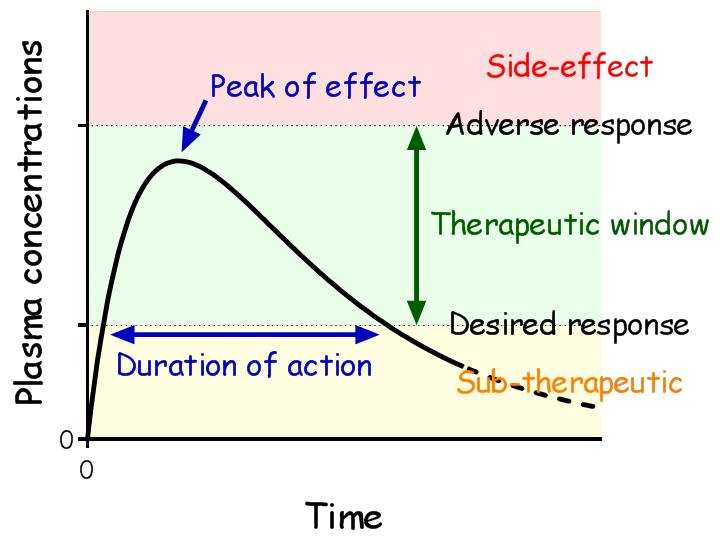
\includegraphics[width=0.7\textwidth]{Images/therapeutic-window.jpg}
	\caption{Plot showing Minimum Toxic Concentration, Minimum Effective Concentration and their relation to the Therapeutic Window \cite{Therapeutic_Index_And_Window}}
    \label{fig:theraputic_window}
\end{figure}

	
In terms of this project, the therapeutic window of many common chemotherapeutic drugs (such as cyclophosphamide) are typically very narrow \cite{cyclophosphamide_details}. As such, it is of high importance to ensure that all cumulative effects as a result of long term exposure to these medications are taken into consideration when modelling the excretion and adsorption of them. This is especially true with respect to going above the MTC of drugs with therapeutic windows which are narrow, as this can result in serious changes in the expected outcome for a patient \cite{Clinical_Pharmacokinetics_and_Pharmacodynamics_Concepts}.

As part of attempts to better characterise the non-linear effects which some drugs can cause after prolonged use, such as deep tissue trapping and long term accumulation, new approaches have recently been developed to aid in modelling these phenomenon \cite{ion_trapping, cumlative_effects}. To date, standard methods of modelling these systems have focused on the use of zero order and first order differential equations \cite{Clinical_Pharmacokinetics_and_Pharmacodynamics_Concepts} in conjunction with compartmental models to track the concentrations of a drug in different kinetically similar parts (or "compartments") of the body (although different compartments have no direct relationship anatomically) \cite{Compartmental_modeling_in_Pharmacokinetics}. These models however, fail to take into account the non-linear elements of the model, and as such the recent research instead attempts to make use of a concept known as fractional-order calculus to model these systems. These fractional order pharmacokinetic systems have a number of benefits over the standard integer order systems. First and foremost is that fractional order pharmacokinetics allows non-linear elements to be taken into account in the model in stark contract to first and zero order systems. Secondly, the fact that fractional order pharmacokinetics, unlike first and zero order pharmacokinetics, take into account an entire weighted history of the system, means that when repeat maintenance doses are given to a patient, the impact of the ``first-pass effect" and use of other techniques like a loading dose may be accounted for in calculations \cite{Clinical_Pharmacokinetics_and_Pharmacodynamics_Concepts}. 

\subsection{Objectives} \label{objectives}

Based on this background, this project has three elements to it. The first of these is to develop a fractional order model capable of simulating fractional order pharmacokinetics in a single compartment system. This will then be used to estimate the order and initial conditions of a given dataset using a least squares methodology. Following on from this, the project has been further developed using Bayesian statistics, through the provision of a set of prior distributions for the estimated parameters which when used help to produce results with higher credibility \cite{statistical_rethinking}. This finally culminates in a system which is capable of using live streamed data to perform the estimations, with new information allowing for updated estimations of noise in the system. 

This work has a number of benefits for industry in terms of its potential applications. In its current state this system will allow for further investigation into new methods of personalising medicine, with the parameters being estimated potentially being able to be used to design specific drug regimens for specific patients. This in turn may allow given fractional order values to be correlated, along with other pieces of patient information such as demographics and other pharmacokinetic parameters with patient outcomes, allowing more for informed decisions around patient treatment.

The developments in this field have not been possible in the past, primarily as a result of the large amount of processing power required to perform the calculations when a large number of steps are estimated. Of course, in the last 30 years a variety of fields have been able to begin making use of Bayesian statistical methods and machine learning as a result rapid improvements in computational abilities.

This document therefore shall outline, over the course of the following pages, the theory, and further define the objectives, methodology and results of this project. These shall be analysed in the context of other research papers which shall be used to provide further insight into the current state of this area of enquiry. Additionally specific details of the software produced shall also be included in this document to act as documentation for any future progress that may occur with respect to this project.

\subsection{Current Literature} \label{current_literature}

To date there have been a selection of papers written which have approached the use of fractional order derivatives in the context of pharmacokinetics. One paper of interest is the International Federation of Automatic Control's \textit{Modeling and administration scheduling of fractional-order pharmacokinetic systems} \cite{Modeling_and_administration_scheduling}. The primary objective of this paper is to identify a numerical method for the simulation of a fractional order system and then to implement this such that the chosen method is used to simulate the pharmacokinetics of a given drug which is confirmed by means of a optimal control problem. 

In terms of the approach taken in this paper, a number of different forms of fractional order derivatives were reviewed. These included the Caputo $\gls{caputo_derivative}$, Riemann-Liouville $\gls{riemann_liouville_derivative}$ and the Gr\"{u}nwald-Letnikov $\gls{grunwald_letnikov_derivative}$ derivatives, which are operators used to form fractional-order differential equations. Upon addressing these and providing definitions the primary focus of the paper is then approached, looking at a variety of methods of solving Fractional order Differential Equations (FDE's) numerically (although it is pointed out that in some cases analytical solutions may exist) \cite{garrappa2015numerical}. 

Across this investigation three primary areas are focused on for solving FDE's: using the s-domain through integer order rational transfer functions approximations, numerical discretised approximations in the time domain, the inverse Laplace transformation solved numerically. The analysis of the different methods of solving an FDE resulted in a number of interesting conclusions that had an impact on the development of this project. For example, the conclusion that solving an FDE system using s-domain methods, whilst capable of providing a reasonably accurate solution, is not a reasonable proposition for a constrained system. This in conjunction with the information that the time domain approximation method highlighted in the paper, which involved the use of a discretised version of the Gr\"{u}nwald-Letnikov derivative, is less dependent on the step size for high precision and is more dependent on having a long history of points.

In addition to this, the next area this paper covered was to design a drug administration schedule using an optimal control problem. The problem as formulated in this paper has a point which should be noted for future consideration in a practical situation. It appears that the formulated cost function has the basic assumption that the parameters of the system are known in some capacity in advance (i.e. the order, initial conditions, etc are already available, thought they may not be precisely known). This is useful to know, given it highlights the novel nature of the work completed in this project, in addition to the fact it also demonstrates a clear use case for the work being completed in this project. 

Another paper which has been published and covers this area of academic work is that of the IFAC Proceedings Volumes, titled \textit{Controlled Drug Administration by a Fractional PID} \cite{Controlled_Drug_Administration}. This paper has the objectives of designing a fractional-order PID controller and evaluating its dynamics characteristics and ability to mitigate noise in the system. In the case of this paper, whereas in others mentioned, discretised forms of the fractional order Gr\"{u}nwald-Letnikov operator were highlighted and used in the process of the paper to highlight differences between solving in time domain and s-domain, this paper specifically utilises the Riemann-Liouville and Caputo operators approximately solved using the Oustaloup filter for the time domain and exactly solved in the frequency domain. 

The primary reasoning in this paper is that the use of fractional order dynamics in the design of the PID system will in of itself help stabilise the concentrations of the example drug used in the process of demonstrating the PID design. Over the course of the paper, it is clear that the use of fractional order dynamics is useful to this end, with high levels of closed loop and external noise rejection and high gain-margin both present in the results for this approach. This is of course demonstrating that the design is capable of acting to provide the necessary characteristics to model drugs that have fractional order dynamics.

Of course one point not covered again in this paper is how the parameters for the fractional order system may be known. It is presumed that the order, and other necessities are previously available to the designer of the PID. Obviously for new drugs this is not true, in addition to the idea that the assumption has been made that the order of the drug is a constant for all situations. This however may not be true, with the potential being present that the drug may act as a different order system depending on the patient (or even depending on the previous concentrations of the drug in a patients system). 


\newpage
\section{Theory}

\subsection{Inspiration} \label{Inspiration}
As shown in Section \ref{current_literature}, the development of the use of fractional order calculus from a purely mathematical construct to one of use in pharmacokinetics is a recent development which has in part been been influenced by the failure of traditional integer order systems to accurately describe the dynamics of certain drugs. The development of the use of fractional order dynamics is also in part related to changes in the computational processing capabilities of many researchers in recent years. Having said this however, another area which has also made significant use of fractional order calculus is control theory \cite{Fractional_order_control, FOC_Basics, control_theory_fractional_applications, fractional_control_tutorial}. Use of fractional order dynamics in control systems has allowed for greater stability within these systems. Additionally it also allows engineers greater control via a wider range of parameters for modelling physical phenomena.

It is therefore unfortunate that despite the common use of this technique in control, the way in which it is used is different than the way in which many other fields would, at least initially, wish to use it. The problem being that outside control, parameter estimation, (with respect to values such as the order and the initial conditions of the system), is a highly useful technique in the context of fractional order systems. This of course resulted in a lack of attention being given to fractional order methods of characterising systems outside control, which was one of the few areas in which the order, and other parameters are selected in advance of their use and left unchanged.

\subsection{Modelling System Dynamics} \label{Modelling_System_Dynamics}

In pharmacokinetic systems, the adsorption, distribution, metabolism, and excretion of drugs is modelled through the use of differential dynamics equations for flow of the drugs between compartments within the body. At the most basic level a compartment model of the human body can consist of a single compartment (known as the central compartment), which typically has its concentrations represented by the concentrations present in blood plasma \cite{Compartmental_modeling_in_Pharmacokinetics, One_Compartment_Open_Model}. The system shown in Figure \ref{fig:single_compartment_model} is an example of this model. 

\begin{figure}[h]

	\begin{center}
	
		\begin{tikzpicture}[scale=1.4]
		
		% Draw Shape
		\draw[->, very thick] (0,0) -- (0, -1);
		\draw[thin] (-1,-3) rectangle (1, -1);
		\draw[->, dashed, very thick] (0,-3) -- (0, -4);
		
		% Labels
		\draw node[scale=10/12] at (1.5, -0.35) {IV Bolus Administration};
		\draw node[scale=10/12] at (1.5, -0.65) {(Zero Order Dynamics)};
		
		\draw node[scale=10/12] at (0, -1.8) {Central};
		\draw node[scale=10/12] at (0, -2.2) {Compartment};
		
		\draw node[scale=10/12] at (1.7, -3.4) {Excretion};
		\draw node[scale=10/12] at (1.7, -3.7) {(Fractional Order Dynamics)};
		
		\end{tikzpicture}
	
	\end{center}
	\caption{Example of a single compartment model of the human body with fractional order dynamics}
    \label{fig:single_compartment_model}
    
\end{figure}

Of course this model is very simple and does not fully describe the infinite complexity that could be gone into with respect to pharmacokinetics in the body. Other models which are typically used in the modelling of drugs include 3 and 7 compartment models, which take into account various different types of tissue in the body with similar dynamical properties. An example of a 3 compartment model involving fractional order pharmacokinetics is shown in Figure \ref{fig:three_compartment_model}.

\begin{figure}[h]

	\begin{center}
	
		\begin{tikzpicture}[scale=1.4]
		
		% Draw Shape
		\draw[->, very thick] (0,0) -- (0, -1);
		\draw[thin] (-1,-3) rectangle (1, -1);
		\draw[->, very thick] (0,-3) -- (0, -4);
		\draw[thin] (-1,-4) rectangle (1, -6);
		\draw[<-, dashed, very thick] (1, -5.25) -- (3, -5.25);
		\draw[->, very thick] (2, -3) -- (1, -4);
		\draw[->, very thick] (1, -4.75) -- (3, -4.75);
		\draw[->, very thick] (0, -6) -- (0, -7);
		\draw[thin] (3,-4) rectangle (5, -6);
		
		% Labels
		\draw node[scale=10/12] at (0, -1.8) {Intestinal};
		\draw node[scale=10/12] at (0, -2.2) {Tract};
		
		\draw node[scale=10/12] at (0, -4.8) {Central};
		\draw node[scale=10/12] at (0, -5.2) {Compartment};
		
		\draw node[scale=10/12] at (4, -4.8) {Tissue};
		\draw node[scale=10/12] at (4, -5.2) {Compartment};
		
		\draw node[scale=10/12] at (1.05, -0.45) {Oral Ingestion};
		
		\draw node[scale=10/12] at (-0.75, -3.4) {Intestinal};
		\draw node[scale=10/12] at (-0.75, -3.7) {Adsorption};
		
		\draw node[scale=10/12] at (2.9, -2.75) {Intravenous};
		\draw node[scale=10/12] at (2.9, -3.05) {administration};
		
		\draw node[scale=10/12] at (2, -4.25) {Integer Order};
		\draw node[scale=10/12] at (2, -4.55) {Dynamics};
		
		\draw node[scale=10/12] at (2, -5.5) {Fractional Order};
		\draw node[scale=10/12] at (2, -5.8) {Dynamics};
		
		\draw node at (-0.75, -6.5) {Excretion};
		
		\end{tikzpicture}
	
	\end{center}
	\caption{Example of a three compartment model of the human body with fractional order dynamics for the drug Amiodarone \cite{kuhlkamp1999effect}}
    \label{fig:three_compartment_model}
    
\end{figure}

One issue that is present in these models however, is that with more than one compartment, modelling the dynamics quickly becomes significantly more complex, particularly if one or more of the compartments has fractional order dynamics governing the flow in or out of it. This is in part because maintaining the conservation of mass of the drug in each compartment becomes highly complex when estimating the order of each dynamics equation, along with other parameters due to the interdependence between each equation. It is for this reason that this project was specifically focussed on modelling the excretion from a single compartment system, as shown in Figure \ref{fig:single_compartment_model}. 

In addition to the modelling of the system via compartmental methods, it is important to note that the dynamical equations which are used to describe the flow of the drug, in the case of the model in \ref{fig:single_compartment_model} out of the body, can be considered to be either fractional, first, or zero order equations. Given the wide variety of different equations which may be used to describe these phenomena, and that they may be of varying order, this paper therefore uses a simple exponential equation to test the methods when programmed and leaves the dynamical equation open to change by the end user.

\subsection{Fractional Order Derivatives and Pharmacokinetics}\label{fod_and_pharmacokinetics}

Fractional Order Differential Equations are a class of differential equation which there has been interest in nearly as long as Integer Order Differential Equations, with it first being mentioned in a letter between Leibniz and L'Hospital in 1695 \cite{the_fractional_calculus}. Since then the earliest systematic studies of the idea began in the early 19th century. 

In modern terms, the primary forms of the fractional order derivative in the context of pharmacokinetics are the Caputo, Riemann-Liouville and the Gr\"{u}nwald-Letnikov derivatives, each of which is slightly different in terms of it's definition. One such difference it that when using the Caputo definition for example, taking the derivative of a constant is in fact 0, compared to the Riemann-Liouville definition for which this is not true. These differences are possible as each definition is applicable to a different situation. Despite these differences however, one element all of these definitions have in common is that they collapse back into the standard definition for a derivative when the order is an integer. 

The reasoning for their use with respect to the field of pharmacokinetics, as partially explained in Section \ref{Modelling_System_Dynamics}, is tied to the ability of fractional order derivatives to take into account an infinite history of a system, not just the local history at a particular point. Another reason which should be noted as significantly important is that the systems in question are fractional order in nature, i.e. they exhibit non-linear fractional order behaviour when they are observed.

Despite the large volume of material in this subject area for the purposes of this project, the primary focus shall be the implementation of the Gr\"{u}nwald-Letnikov (GL) derivative. The reasoning behind this is primarily related to the ability to easily discretise the GL derivative. This ability means that this method can be used to approximate fractional order differential equations.

\subsection{Gr\"{u}nwald-Letnikov Derivatives} \label{gl_derivatives}

Gr\"{u}nwald-Letnikov (GL) derivatives are fundamentally an extension of the most basic numerical method of obtaining first order derivatives, Euler's method, such that the order being solved can be a non-integer value \cite{the_fractional_calculus, euler1794institutiones}. Given some function $\gls{general_function}$, with a derivative of $\gls{first_order}$, dependent variable $\gls{general_dependent_variable}$, and a step of $\gls{time_step}$, Euler's method is given by the equation,
\begin{equation}\label{eulers_method}
	f^{\prime}(x) = \lim_{h \to 0} \frac{f(x)-f(x-h)}{h} \approx \frac{f(x)-f(x-h)}{h},
\end{equation} 
provided that $\gls{time_step} > 0$ and is sufficiently small. It can be noted at this point that assuming that $\gls{general_function}$ is continuously differentiable, Equation \ref{eulers_method} is simply a first order approximation using Taylors theorem. 

Therefore, using Equation \ref{eulers_method}, a second order derivative of a function, as given by $\gls{second_order}$ can also be obtained through iteratively applying this method. Doing so gives rise to the equation,
\begin{equation}\label{second_order}
	f^{\prime\prime}(x)= \lim_{h \to 0} \frac{f^{\prime}(x)-f^{\prime}(x-h)}{h} \approx \frac{f^{\prime}(x)-f^{\prime}(x-h)}{h},
\end{equation}
which of course can be expanded out and simplified such that no intermediate step of calculating the first order derivative is required,
\begin{equation}\label{second_order_expanded}
	f^{\prime\prime}(x) = \lim_{h \to 0} \left\{\frac{\left(\frac{f(x)-f(x-h)}{h}\right)-\left(\frac{f(x-h)-f(x-2h)}{h}\right)}{h}\right\},
\end{equation}
\begin{equation}\label{second_order_simplified}
	f^{\prime\prime}(x) = \lim_{h \to 0} \left\{\frac{1}{h^{2}}\left\{f(x)-2f(x-h)+f(x-2h)\right\}\right\},
\end{equation}
doing this again for the third order derivative $\gls{third_order}$, gives rise to this equation,
\begin{equation}\label{third_order}
	f^{\prime\prime\prime}(x)= \lim_{h \to 0} \frac{f^{\prime\prime}(x)-f^{\prime\prime}(x-h)}{h} \approx \frac{f^{\prime\prime}(x)-f^{\prime\prime}(x-h)}{h},
\end{equation}
simplified, 
\begin{equation}\label{third_order_simplified}
	f^{\prime\prime\prime}(x) = \lim_{h \to 0} \left\{\frac{1}{h^{2}}\left\{f(x)-3f(x-h)+3f(x-2h)-f(x-3h)\right\}\right\},
\end{equation}
which allows a pattern that is forming to be observed. The binomial expansion that is present in the simplified forms of the equations Equation \ref{second_order_simplified} and Equation \ref{third_order_simplified} mean that these can therefore be defined in terms of a general equation that can be used for obtaining any $\gls{n}$ order derivative $\gls{general_order_derivative}$ of a given function $\gls{general_function}$,
\begin{equation}\label{third_order_generified}
	f^{\prime\prime\prime}(x) = \lim_{h \to 0} \left\{\frac{1}{h^{3}}\sum_{j=0}^{3} (-1)^{j} {3 \choose j} f(x-jh)\right\},
\end{equation}
\begin{equation}\label{general_order}
	f^{(n)}(x) = \lim_{h \to 0} \left\{\frac{1}{h^{n}}\sum_{j=0}^{n} (-1)^{j} {n \choose j} f(x-jh)\right\}.
\end{equation}

Equation \ref{general_order} therefore is the general equation for obtaining a derivative of any order. The final step which results in the GL derivative is to extend the binomial coefficient operator such that instead of using the factorial in the calculation, the $\Gamma$ function is used in its place. This means using the identity $\Gamma(\Omega+1) = \Omega!$, for any real number $\Omega$. Doing this means that the binomial operator is replaced with,
\begin{equation}\label{extended_binomial}
	{\alpha \choose j} = \frac{\Gamma(\alpha + 1)}{j!\Gamma(\alpha-j+1)}.
\end{equation}

Upon replacement, the only remaining element left to change is that the value of $n$ as the upper limit in the sum must be changed so it is still an integer value. To do this, the floor of the current point $x$, divided by the time step (i.e. how many previous points in history there are), must be used. This means that the overall GL derivative for an order of $\gls{fractional_order}$ is given by,
\begin{equation}\label{gl_order}
	^{gl}D^{\alpha}_{x}f(x) = \lim_{h \to 0} \left\{\frac{1}{h^{\alpha}}\sum_{j=0}^{\lfloor\frac{x}{h}\rfloor} (-1)^{j} {\alpha \choose j} f(x-jh)\right\}.
\end{equation}

\subsection{Discretisation And Computability}

Based on the equations for the GL derivative highlighted in Section \ref{gl_derivatives}, the first step to allow the computability of the function is to define the extended form of the binomial coefficient operator in such a way as to allow a computer with a finite number of bits to be able to calculate it. To do this, the following equation may be used instead of Equation \ref{extended_binomial}, as the use of Gamma function means in most cases it use is not practical. The equation,
\begin{equation}\label{computable_extended_binomial}
	{\alpha \choose j} = \prod_{i=0}^{j-1}\frac{\alpha-1}{i+1}.
\end{equation}
can therefore be substituted in its place \cite{Fractional_calculus_in_pharmacokinetics}. 

Having said this, to have the ability to compute the GL derivative, it must be discretised. As the GL method is based on a numerical method already, this is trivial. Equation \ref{gl_order} needs only be moved from the continuous domain of $x$ to a discrete domain defined by a step of $\gls{time_step}$ in order to become discretised, with an appropriately small value of $h$ allowing near approximation of the original function. To index each time step, an index $\gls{time_step_index}$ is used, such that $k=\frac{x}{h}$ where $x$ is the current point in the dependent variable and the discrete fractional order differential equation is given by $^{gl}D^{\alpha}_{x}f(x) = z(f)$, meaning the new equation shall be, 
\begin{equation}\label{gl_semi_ddiscretised_order}
	^{gl}D^{\alpha}_{x}f(x) \approx \frac{1}{h^{\alpha}}\sum_{j=0}^{\lfloor\frac{kh}{h}\rfloor+1} (-1)^{j} {\alpha \choose j} f(kh - jh + h) = z(f(kh)),
\end{equation}
\begin{equation}\label{gl_discretised_order}
	 h^{\alpha}z(f_{k}) = {\alpha \choose 0} f_{k+1} + \sum_{j=0}^{k+1} (-1)^{j} {\alpha \choose j} f_{k - j + 1}
\end{equation}

The final step to allow for this to be used in running a simulation is now to rearrange the equation such that the solution to the fractional order differential equation is the subject. To do this, first, since ${\alpha \choose 0}$ is always 1 it can be removed, next Equation \ref{gl_discretised_order} can be rearranged to give,
\begin{equation}\label{gl_solution}
	f_{k+1} = h^{\alpha}z(f_{k}) - \sum_{j=0}^{k+1} (-1)^{j} {\alpha \choose j} f_{k - j + 1}.
\end{equation}

This form of the GL Method can now be used to solve fractional order pharmacokinetics equations, where $f = x$ (i.e. the concentration), $x = t$ (i.e. the time) and $z = \phantom{}^{gl}D^{\alpha}_{x}x(t)$ (i.e. a fractional order dynamics equation) in pharmacokinetics. This of course means the equation is therefore written as,
\begin{equation}\label{gl_pk_solution}
	x_{k+1} = h^{\alpha}\phantom{ }^{gl}D^{\alpha}_{x}x(t_k) - \sum_{j=0}^{k+1} (-1)^{j} {\alpha \choose j} x_{k - j + 1},
\end{equation}
with a bound for the order, $\alpha$, of $0 < \alpha \leq 1$, as to have an alpha greater than one would make no physical sense as it could cause negative concentrations \cite{Fractional_calculus_in_pharmacokinetics}.

\subsection{Estimation}

In order to be able to fit parameters to allow for the estimation of values, the cost function for the optimisation problem must be formed. In terms of this project, initially a version of the least-squares method was used to get an idea how good estimating the parameter values may be given a perfect model with no error or noise, and a non-sparse dataset which has moderate to high levels of measurement noise. To do this, the cost function, Equation \ref{cost_function_one} was implemented, where the sum squared error $\epsilon$ was calculated across $k$ data points $y_{n}$ and the estimations for a given set of model parameters, $x_{n}$, where $n$ is the index in both cases. This is of course subject to the model $F_{t}(x_{0} \dots x_{t}, \alpha, \theta)$, where the finite history, $\alpha$ and $x_{0}$ are used to calculate the solution to the fractional differential equation as the order and initial condition respectively and $\theta$ represents any other parameters in the system, thus giving,
\begin{subequations}
	\begin{align}\label{cost_function_one}
		\operatorname{Minimise} \epsilon(x_{0} \dots x_{t}, \theta) &= \sum_{t=0}^{k} (y_{t}-x_{t})^{2},
	\intertext{subject to:}
		x_{t} &= F_{t}(x_{0} \dots x_{t-1}, \alpha, \theta), \text{ for } t = 1 \dots k,\\
		x_{t} &\geq 0,\\
		\alpha &> 0,\\
		\theta &> 0.
	\end{align}
\end{subequations}

This method in practice works very well, however it makes an assumption that the model that is used is perfect, and that the dataset can exactly fit this model. To take into account estimation noise $w_{t}$ which may be present in the system, the cost function may be updated,
\begin{subequations}
	\begin{align}\label{cost_function_two}
		\operatorname{Minimise} \epsilon(x_{0} \dots x_{t}, \theta) &= \sum_{t=0}^{k} (y_{t}-x_{t})^{2} + w_{t}^{2},
	\intertext{subject to:}
		x_{t} &= F_{t}(x_{0} \dots x_{t-1}, \alpha, \theta) + w_{t}, \text{ for } t = 1 \dots k,\\
		x_{t} &\geq 0,\\
		\alpha &> 0,\\
		\theta &> 0.
	\end{align}
\end{subequations}

Passing these cost functions into an optimisation algorithm such as the L-BFGS-B algorithm \cite{L_BFGS_B_Method} or a particle swarm algorithm \cite{wang2018particle} will allow for an optimum solution to be found easily. The only important element regarding the optimisation algorithm to take into account is the ability to place box constraints on the parameters being optimised such as to avoid clearly illogical values such as negative concentrations.

Once optimum values have been achieved, the process can be ran a significant number of times (simulating multiple experimental datasets with different additive noise), to perform a Markov Chain Monte Carlo simulation to allow the production of probability distribution functions for the estimated parameters. This is done to check the system for its ability to withstand measurement noise and to see how estimations vary with different levels of noise.

This concept of characterising noise and response to noise and variation in the estimated parameters therefore leads onto utilising a Bayesian statistical methodology to allow prior knowledge of the noise and characteristics associated with each parameter to be taken into account. For the value of $\alpha$ when estimating it for a whole dataset, it will likely be best to use a beta distribution for the prior, as this allow for values near the extremes to be less likely (as these values would suggest that the dynamics are not in fact fractional but is likely closer to integer order dynamics). Additionally, the distribution of the initial condition $x_{0}$ is considered to be normally distributed around a mean of a high value as values close to zero are unlikely for this as the concentration when excreting must always go from high to low. The sources of noise in this system are all presumed for now to be normally distributed, however experimental data and information regarding the measurement tools will allow this to change once more prior information is available. 

Using these priors, the cost function highlighted in Equation \ref{cost_function_two} can be modified to obtain a posterior distribution for each parameter which should have an improved credibility interval. The updated cost function also takes into account estimation noise $w_{t}^{\alpha}$, $w_{t}^{\theta}$, and $w_{t}$ as well as measurement noise $v_{t}$ which is present in the experimental dataset. 

The three distributions which are to be used in this updated cost function are the normal, beta and exponential distributions. Putting these into log form for the cost function is a simple process. For the normal distribution, the probability density function is defined by the following equation where $\mu$ is the mean, $\sigma$ is the standard deviation, and x is the variable that is normally distributed, 

\begin{equation}\label{pdf_normal}
	p_{x}(x) = \frac{1}{\sqrt{2\pi}\sigma} \exp{(-\frac{1}{2}(\frac{x-\mu}{\sigma})^{2})},
\end{equation}

As we have the assumption any noise present in the system is unbiased the mean can be assumed to be 0. This gives rise to a new equation which the log is taken of, before one of the rules of logarithms is applied to separate the product term in the equation,
\begin{equation}\label{unbiased_log_pdf_normal}
	-\ln(p_{x}(x)) = \log{\frac{1}{\sqrt{2\pi}\sigma}} + \log{\exp{(-(\frac{x}{2\sigma})^{2})}},
\end{equation}
As the first term in the sum is a constant it can be disregarded, leaving the second term which can be simplified again as the log and exponent cancel out. This means the prior for the normally distributed parameters in the system is able to now be given by,
\begin{equation}\label{unbiased_log_pdf_normal}
	-\ln(p_{x}(x)) = (\frac{x^{2}}{2\sigma}).
\end{equation}
In addition to this, the exponential distribution is used. This is again, simple to write logarithmically, with the original probability density function being,
\begin{equation}\label{unbiased_log_pdf_normal}
	p_{x}(x) = \gamma\exp(-\gamma x),
\end{equation}
where the parameter $\gamma$ is a parameter set by the user. To write this in terms of a log, the rule of logs regarding product terms is again used to remove a $\gamma$ term as a constant, before again the log cancels out with the exponential, leaving,
\begin{equation}\label{unbiased_log_pdf_normal}
	\ln{p_{x}(x)} = -\gamma x.
\end{equation}
The final distribution used in this cost function shall be the beta distribution, which is defined by two parameters, a and b. The probability density function for this distribution is simple to understand, and as such again is simple to write in terms of a logarithmic formulation. The function is,
\begin{equation}\label{unbiased_log_pdf_normal}
	p_{x}(x) = \frac{x^{a - 1}1-x^{b - 1}}{\frac{\Gamma(a) \Gamma(b)}{\Gamma(a+b)}}.
\end{equation}

Once again, the first step in converting this to a logarithm is to use one of the rules of logs to separate the numerator and denominator from each other. This allows the denominator to be removed as a constant. Following this, again using the rule of logs regarding products, the numerator can be separated out into two different terms being summed,
\begin{equation}\label{unbiased_log_pdf_normal}
	\ln{p_{x}(x)} = \ln{x^{a-1}} + \ln{(1-x)^{b-1}}.
\end{equation}

The final step is then to use the log power rule to remove the power terms, giving the following,
\begin{equation}\label{unbiased_log_pdf_normal}
	\ln{p_{x}(x)} = (a-1)\ln{x} + (b-1)\ln{1-x}.
\end{equation}

Using these distributions and substituting in estimated parameters instead of x, the cost function is therefore,
\begin{subequations}
	\begin{align}\label{cost_function_three}
		\operatorname*{Minimise}_{\alpha, \theta, w_{t}, w_{t}^{\alpha}, w_{t}^{\theta}, v_{t}} &\sum_{t=0}^{k} (\frac{w_{t}}{\sigma_{w}}^{2}+\frac{w_{t}^{\alpha}}{\sigma_{w}^{\alpha}}^{2}+\frac{w_{t}^{\theta}}{\sigma_{w}^{\theta}}^{2}+\frac{v_{t}}{\sigma_{v}}^{2}) \notag\\
		&- ((a-1)\ln(\alpha)+(b-1)\ln(1-\alpha)) \notag\\
		&- (\gamma x_0),
	\intertext{subject to:}
		x_{t} &= F_{t}(x_{0} \dots x_{t-1}, \alpha, \theta) + w_{t}, \text{ for } t = 1 \dots k,\\
			\alpha_{t+1} &= \alpha_{t} +  w_{t}^{\alpha},\\
			\theta &= \theta + w_{t}^{\theta},\\
			y_{t} &= x_{t} + v_{t},\\
			x_{t} &\geq 0,\\
			\alpha &> 0,\\.
	\end{align}
\end{subequations}

These methods of course require a full dataset of nearly continuous data to work, however a small change in the method of performing the minimisation can correct for this, with the moving horizon estimate one option that may be used for a continuous stream of data for which is it not possible to have a full history stored without memory issue. Another option may be to simply perform the minimisation over the data points which are present in the experimental data, i.e. instead of a sum over all points from 0 to the maximum time at steps of size $h$, simply index the times which measurements were taken and compare these to the estimated values. The use of the a priori methodology should also help here, with details of the distribution for each parameter helping to guide the maximum likelihood method which has been used.


\newpage
\section{Software Documentation}

\subsection{Features}

The developed code for this project has several features which are of note. The primary feature is the ability of the developed code to estimate the order and initial conditions of highly noisy data with reasonable accuracy when a correct model is used. For noise characterisation as well the system performs well, being able to take a noisy dataset, and reconstruct it using a given model with both the main system and the noise in the system. Additionally, the ability to run a Monte Carlo simulation or estimate parameters for a population is also present. The ability to perform estimations on noisy datasets is further improved upon by the ability of the system to also do this with sparse datasets with reasonable accuracy.

Further to this, the program has the ability to easily customise both the dynamics of the system being modelled, and the priors for each of the variables being estimated. These customisable functions are listed at the top of one of the main project file, with clear function names. The end user only needs information on the priors for each parameter to customise the cost function to their own needs.

\subsection{Code Structure} \label{code_structure}

The structure of the code has been developed to be as simple as possible. There are currently 3 primary classes which exist in the code base for consumption. One which has the primary focus on calculating solutions to fractional order derivative, another which again has the focus of calculating fractional order derivatives (although this class is written in C++ and so has limited features when called from Python compared to the pure python version), and an optimisation class which fits a provided dataset to parameters for a model. 

Simply put, the optimiser class takes one of the GLMethod class objects, a dataset, and will return the parameter estimations for the given dataset. In addition it also has the ability to run a Monte Carlo simulation, or perform estimations of parameters for experimental information from a population.

Additionally there is also another class which is not meant for use as a public class, however was still necessary. That is, an iterator for calculating the binomial coefficient needed, as re-calculation of previous coefficients was an incredibly slow process to complete for every new point.

\subsection{Design Choices}

Within the code base a number of design choices have been made for both simplicity of use and for optimisation.

The most obvious decision to be is regarding the language choice for programming the system. Python was chosen due its versatility within the machine learning and scientific community, however it proved too slow for large histories when calculating new points. As a result, the slowest element of the system (namely using the GL method class), was re-written in C++ with a Python wrapper. This results in significant improvements in speed, with around a 52 times performance improvement over simply using python and numpy. This is likely in part as a result of numpy being optimised primarily for matrix and parallelizable operations.

Additionally, the entire structure of the GL Method object is hierarchical, with a function to calculate a solution to any FDE, calling function which will solve FDE's up to the first order, which in turn calls a function which will solve for a point solution. The benefit of this structure is two fold. Firstly it allows for a simpler process of debugging, as every function is compartmentalised. It however also has the side effect of making the class more versatile and potentially useful in the future as well.

Another design choice which was taken in this project was to make use of the scipy library's optimisation functions. This was due to the ease with which box bounds could be added to a problem, in addition to providing access to a wide variety of different optimisation algorithms. 


\newpage
\section{Results, Testing and Discussion}

The results of running a number of tests on this project have been highly successful. In terms of the functionality of estimating purely just the order and initial conditions of the system, the ability of the system to do this can be demonstrated using both the least squares form highlighted in Equation \ref{cost_function_one} and the method which makes use of a bayesian approach in Equation \ref{cost_function_three}. 

In Figure \ref{fig:noise_estimation_simulation} the result of running a test on the system can be seen. The testing methodology was simple in nature, comprising of generating a dataset which was fractional order in nature using a predetermined model with the equation $-5\exp(x)$, an order of 0.7 and initial conditions of 1.0. This dataset was then subject to the addition of normally distributed noise with a standard deviation of 0.1 and mean of 0, before finally being thinned from a full set of data at regular steps of 0.01 down to 50 data points at random intervals. This dataset was then given to the estimator which attempted to reconstruct the parameters which could then be used to estimate the values between measurements.

\begin{figure}[h]
	\centering
	\includegraphics[width=0.55\textwidth]{Images/EstimatedSystem1650946990.png}
	\caption{Plot of the result of performing parameter and noise estimation on a sparse dataset}
    \label{fig:noise_estimation_simulation}
\end{figure}

The same methodology was also able to be used on the least squares form of the system with the slight modification of reducing the number of data points available again to give it only 20. This gave rise to the plot shown in Figure \ref{fig:least_squares_estimation_simulation}. 

\begin{figure}[h]
	\centering
	\includegraphics[width=0.55\textwidth]{Images/EstimatedSystem1650986363.png}
	\caption{Plot of the result of performing parameter estimation on a sparse dataset using a least squares methodology}
    \label{fig:least_squares_estimation_simulation}
\end{figure}

One point to note however is that whilst the results shown are very good, there was some variance between consecutive runs of the estimator with different noise values. Running a Monte Carlo simulation where 12000 estimations were performed, each with new random noise allowed for characterisation of this variance. The plots shown in Figures \ref{fig:least_squares_estimation_monte_carlo_simulation_alpha} and \ref{fig:least_squares_estimation_monte_carlo_simulation_x_0} demonstrate however that the system is remarkably robust at estimating parameters consistently, with noise only resulting in a maximum deviation from the true value of 0.008 for the order $\alpha$ and around 0.3 for the initial conditions.

\begin{figure}[h]
	\centering
	\includegraphics[width=0.55\textwidth]{Images/EstimatedAlphaValues1650956653.png}
	\caption{Plot of the result of performing parameter estimation for the order, $\alpha$ of a system using a Monte Carlo on a sparse dataset using a least squares methodology with randomly added noise}
    \label{fig:least_squares_estimation_monte_carlo_simulation_alpha}
\end{figure}

\begin{figure}[h]
	\centering
	\includegraphics[width=0.55\textwidth]{Images/EstimatedInitialConditionValues1650956669.png}
	\caption{Plot of the result of performing parameter estimation for the initial conditions of a system using a Monte Carlo method on a sparse dataset using a least squares methodology with randomly added noise}
    \label{fig:least_squares_estimation_monte_carlo_simulation_x_0}
\end{figure}

Interestingly, part of the reason behind the difference in the standard deviation of $\alpha$ and the standard deviation of the initial condition estimation appears to be tied to the dependence of the system on having sufficient numbers of data points early in the dataset to aid estimation. This can be seen in Figure \ref{fig:poor_initial_condition_estimate}.

\begin{figure}[h]
	\centering
	\includegraphics[width=0.55\textwidth]{Images/EstimatedSystem1650947998.png}
	\caption{Plot showing low number of data points in early period of dataset and the associated estimated system}
    \label{fig:poor_initial_condition_estimate}
\end{figure}

Another important feature of the developed system is the ability to estimate measurement and estimation noise. In Figure \ref{fig:measurement_noise}, the distribution of measurement noise for a single sparse dataset is shown. The dataset did not have many points available to the system, however despite this it appears to have done a good job to estimating that the distribution was normally distributed, with a mean of 0 and a standard deviation of 0.1, as shown by the peak at 0 that rolls off on either side of the histogram. 

\begin{figure}[h]
	\centering
	\includegraphics[width=0.6\textwidth]{Images/EstimatedMeasurementNoise1650985937}
	\caption{Plot showing estimated measurement noise which is present in the system}
    \label{fig:measurement_noise}
\end{figure}

Another point to take into account in this system is the performance in terms of speed. Initially the function for calculating the solution to a fractional order derivative took an exceptionally long time. In Table 1 the improvement in speed that came from using C++ code in a python wrapper can be clearly seen. This change in speed made the ability to run the Monte Carlo significantly more realistic, in addition to making the estimations of noise in a dataset a viable option, as previously the slow speeds made it unrealistic to use.


\begin{center}
\begin{tabular}{||c c c c||}
 \hline
 Number Of Points & C++ Time & Python Time & Performance Improvement Factor \\ [0.5ex] 
 \hline\hline
500 & 0.0267s & 1.335s & 49.918 \\ [1ex] 
 \hline
5000 & 2.199s & 114.397s & 52.033 \\ [1ex] 
 \hline
50000 & 20.898s & 1143.155s & 54.701 \\ [1ex] 
\hline
\end{tabular}
\end{center}
\caption{Table 1: Table showing respective times taken in second for 2 forms of the code to solve the GL Derivative and the resultant speed improvement}


\newpage
\input{Discussion.tex}

\newpage
\section{Conclusion}

The results of the testing completed on the system demonstrates its effectiveness at performing the desired estimations. In addition to the surprisingly high tolerance of the system to having a small number of data points and high levels of noise to work with, it should be noted that the ability to perform these estimations precisely for a sparse dataset is at its optimum when at the very least, the dataset has more measurements taken around the early stage in the experimental procedure.

Overall, the practical implications of the development of this system are significant in the field of pharmacokinetics. It should significantly help with the process of drug discovery with respect to drugs that exhibit non-linear pharmacokinetics by allowing the easy identification of the order of the pharmacokinetic dynamics. Additionally, the bayesian approach which has been utilised also has the potential to provide significant improvements to patient care through the ability to utilise prior information regarding the patient and the distributions of parameters associated with their demographics to achieve narrower credibility intervals.

\newpage
\bibliographystyle{IEEEtran}
\bibliography{Bibliography.bib}

\newpage
\begin{center}
   \vspace*{1cm}
   \vfill
   \Huge
   \textbf{Appendix}
   \vfill
\end{center}
\phantom{-}
\section{Results}

\begin{figure}[h]
	\centering
	\includegraphics[width=0.5\textwidth]{Images/EstimatedPopulationAlphaValues1651046027.png}
	\caption{Plot showing variation in the estimations of order $alpha$ when performing noise characterisation and estimation for a system with order 0.7}
\end{figure}

\begin{figure}[h]
	\centering
	\includegraphics[width=0.5\textwidth]{Images/EstimatedPopulationInitialConditionValues1651046042.png}
	\caption{Plot showing variation in the estimations of initial conditions when performing noise characterisation and estimation for a system with initial condition of 1.0}
\end{figure}


\end{document}
